\documentclass{article}

\usepackage{amsmath}
\usepackage{graphicx}
\usepackage{courier}
\usepackage{multicol}
\usepackage{microtype} %required to fix courier linebreaking issues
\usepackage{hyperref} % make references into links
\usepackage{amsfonts}
\hypersetup{colorlinks=true, linkcolor=blue} %make them pretty links
\usepackage[all]{hypcap} %make them link to the right place
\graphicspath{{spark_images/}{png/}}

\begin{document}
	\title{AC290r.1: Influence Maximization Problem}
	\author{Stephen Carr and Charles Liu}
	\date{\today}
	\maketitle
	
	\section{Introduction}
	
	\subsection{Goal and Motivation}
	
	From a marketing perspective, social networking sites provide a large number of users with personal and persuasive information regarding products. With limited resources, one would want to know how to reach advertisement to the most number of people in this personalized manner. This problem can be reduced to a graph, where each user is a node and each relationship between users is represented by an edge with some weight to indicate the strength of their relationship. Which user, or set of users, has the ability to spread your product to the greatest number of potential customers?
	
	\subsection{Data set}
	
	The user network of the online restaurant reviewing site Yelp is used in this study. Each account represents the node, and the edges are to be generated by looking at which accounts posted reviews of the same restaurant within a certain time period of one another. This information (the user, their total number of reviews, and how many reviews they have written within 1 month of another user) was pulled from the Yelp site, turned into a library format, and then imported into a python development environment using network x. For most of the prototyping of a solution, a subset of the North Carolina network was taken, which consisted of 240 nodes and ???? edges.
	
	\subsection{Independent Cascade, $I(s)$}
	
	We start with a set of nodes $s = \{n_1,n_2,...,n_k\}$ and wish to find the number of nodes which are activated through our probabilistic network of influence. So for each node $n$ in our original set $s$, we look at all nodes connected to $n$ by an edge and use the beta distribution to determine if the connected node $n_c$ activates (we ignore $n_c$ if it is already activated). The beta distribution $\boldsymbol{B}$ is given by:
	\begin{equation}
	\boxed{
			\int_{-\infty}^{\infty} \frac{dx}{\boldsymbol{B}(\alpha,\beta)}x^{\alpha-1}(1-x)^{\beta - 1} = 1
		}
	\end{equation}
	Where $\beta$ is taken to be the number of reviews node $n_c$ has written within one month of node $n$ writing a review of the same restaurant, and $\alpha$ is taken to be the number of reviews $n_c$ has written. A uniform distribution is taken between $0$ and $1$ and if its value is less than $\boldsymbol{B}(\alpha,\beta)$ then $n_c$ activates and we repeat the same process for neighbors of $n_c$. This recursive process continues until either all nodes are activated or no activated nodes are left in the loop. The number of nodes activated is called $I(s)$.
	
	
	\section{Stochasticity}
	
	\subsection{Averaged Trial Function, $f_N(s)$}
	
	Since each step of the independent cascade is a random sampling of the beta distribution, there is no guarantee that two different measurements of $I(s)$ will be the same, or even "close" to one another, as seen in \ref{fig:Inf_1000}. 
	
	\begin{figure}[h!]
		\centering
		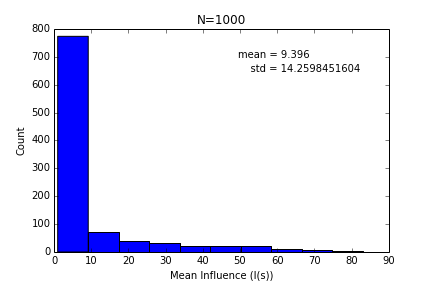
\includegraphics[width=100mm]{N1000_influence.png}
		\caption{Histogram of values $I(s)$ over 1000 iterations for a fixed node in the 240 North Carolina subgraph.}
		\label{fig:Inf_1000}
	\end{figure}
	
	Because of this, we must define a new measurement of a node's influence, namely its mean over $N$ samples:
		\begin{equation}
		\boxed{
			f_N(s) = \frac{1}{N}\sum_1^N I(s)
		}
		\end{equation}
		
		
		
	\subsection{Properties of $f_N(s)$}
	Obviously we cannot take $N$ arbitrarily large, so we must understand how $f_N$'s properties vary with $N$. Taking a 240 node subset of North Carolina, we obtain the following relationship between $N$ and the standard deviation of $f_N$ in \ref{fig:lambda}.
	
		\begin{figure}[h!]
			\centering
			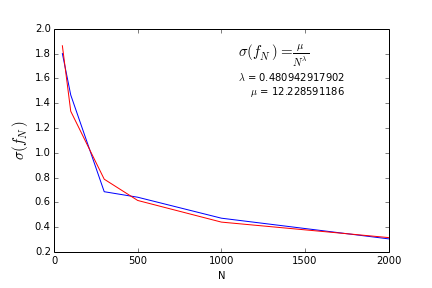
\includegraphics[width=100mm]{lambda_regression.png}
			\caption{Fitted regression for the standard deviation of $f_N(s)$. This was with 100 trials for each N value. The blue line is the simulation, while the red line is the fitted relationship.}
			\label{fig:lambda}
		\end{figure}
			
	
	\section{Greedy Algorithm}
		Although this problem is inherently non-linear in its parameters (the starting set of nodes), we can try to solve it in a linear way. This is called the "Greedy Algorithm":
		Given nodes $s_i = \{n_1, n_2,..., n_i\}$, check every remaining node to find node ${n_{i+1}}$ that maximizes $f(s_{i+1})$ where $s_{i+1} =  \{n_1, n_2, ..., n_i, n_{i+1}\}$.

	\subsection{NC\_Mini}

		For $k = 3$ on our 240 node North Carolina subset we found variation in the maximal $I(s)$.

		\begin{table}[h!]
		  \begin{center}
		    \caption{100 runs with k=3, t=10}
		    \label{tab:table1}
		    \begin{tabular}{|c|c|c|c|} 
		      \hline
		      N & min & max & $\lambda$\\
		      100  & 42.98 & 51.16 & 0.840\\
		      300  & 44.73 & 49.24 & 0.908\\
		      500  & 45.04 & 47.696 & 0.944\\
		      1000 & 45.66 & 47.31 & 0.965\\
		      \hline
		    \end{tabular}
		  \end{center}
		\end{table}

		{\centering
		\hspace*{-3.75cm}
		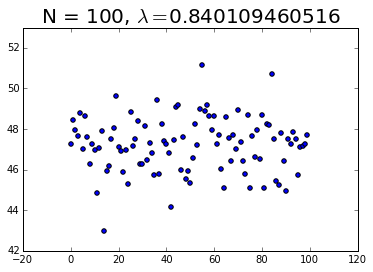
\includegraphics[scale=0.55]{100_scatter}
		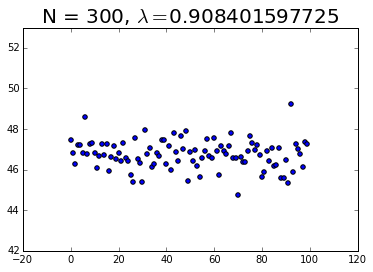
\includegraphics[scale=0.55]{300_scatter}
		\hspace*{-3.75cm}
		\vspace*{1.25cm}
		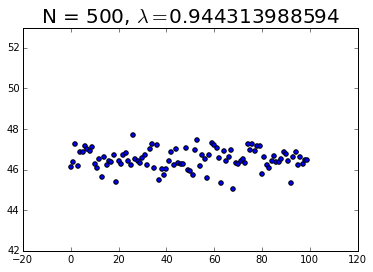
\includegraphics[scale=0.55]{500_scatter}
		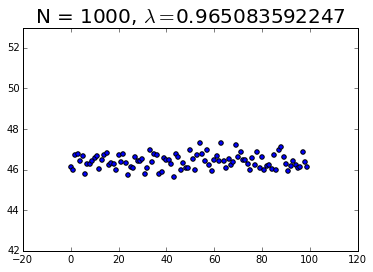
\includegraphics[scale=0.55]{1000_scatter}	
		\hspace*{-3.75cm}
		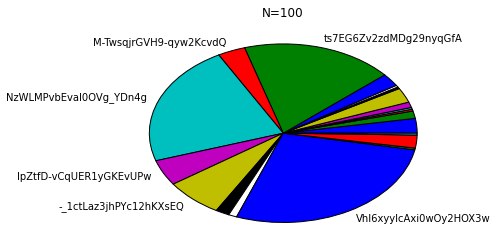
\includegraphics[scale=0.4]{100_pie}
		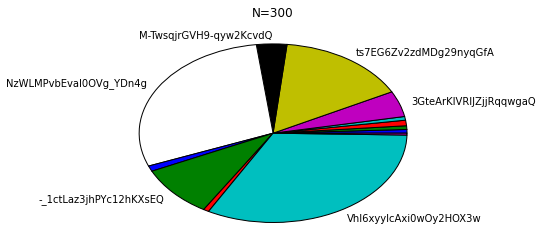
\includegraphics[scale=0.4]{300_pie}
		\hspace*{-3.75cm}
		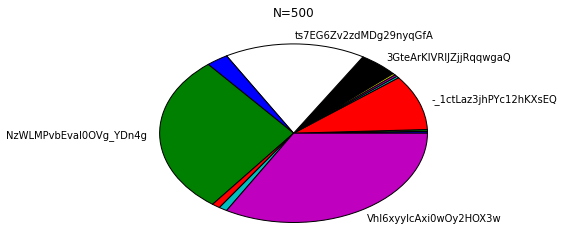
\includegraphics[scale=0.4]{500_pie}
		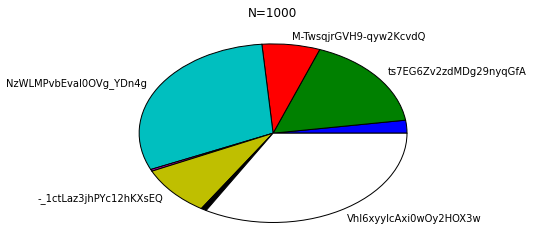
\includegraphics[scale=0.4]{1000_pie}
		\par}	
		\newpage
		

		The scatterplots of the max values over the 100 trials show the convergence of results as N increases. We can similarly see the convergence through the number of nodes selected over the course of our trials. More formally, let $\mathbb{N}_i$ represent the set of nodes returned over all 100 trials of $N=i$. We have

		\begin{equation}
		\boxed{
			 \mathbb{N}_i \subset \mathbb{N}_j, i > j\\
		}
		\end{equation}

	\subsection{NC\_Full}

		We wanted to do the same analysis with respect to the depth of search. For the larger NC\_full graph, our results were:

		\begin{table}[h!]
		  \begin{center}
		    \caption{15 runs with k=3, N=50}
		    \label{tab:table2}
		    \begin{tabular}{|c|c|c|c|} 
		      \hline
		      t & min & max & $\lambda$\\
		      1  & 1465.32 & 1504.28 & 0.9741\\
		      4  & 8453.82 & 8480.96 & 0.9968\\
		      7  & 8966.66 & 8980.06 & 0.9985\\
		      10 & 8985.16 & 8998.66 & 0.9985\\
		      \hline
		    \end{tabular}
		  \end{center}
		\end{table}

		{\centering
		\hspace*{-3.75cm}
		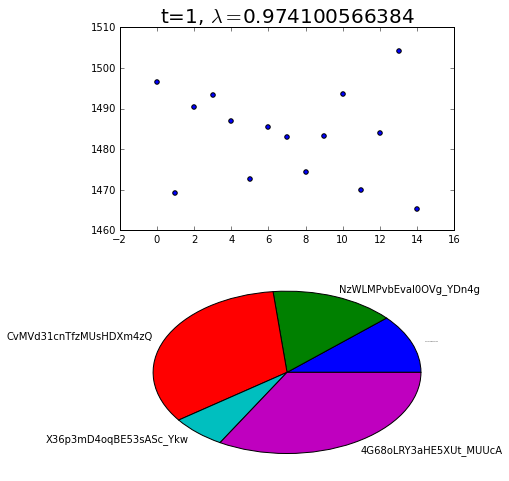
\includegraphics[scale=0.4]{full_1t}
		\hspace*{1cm}
		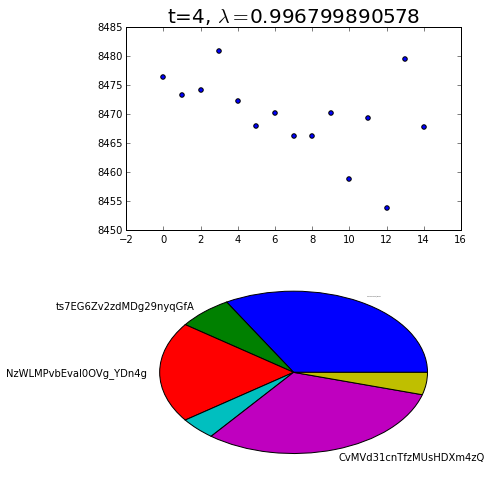
\includegraphics[scale=0.4]{full_4t}
		\hspace*{-3.75cm}
		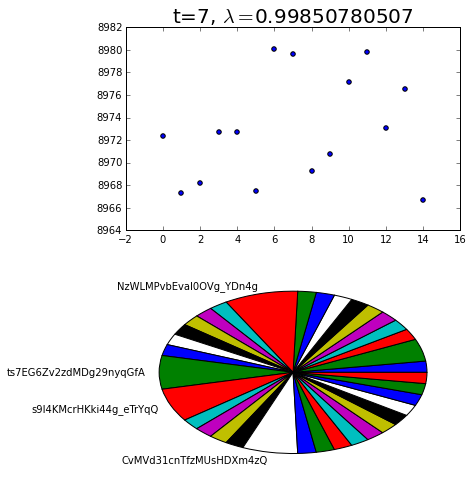
\includegraphics[scale=0.4]{full_7t}
		\hspace*{2cm}
		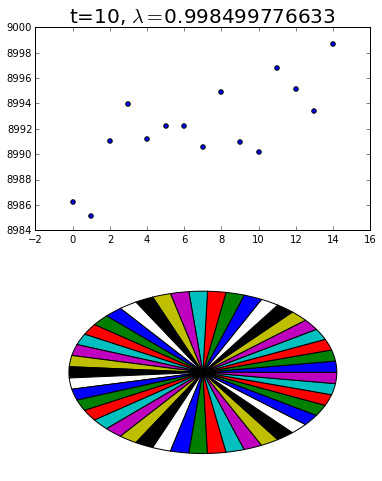
\includegraphics[scale=0.4]{full_10t}
		\par}	
		
		Due to computational limitations, we were only able to run 15 trials for each depth. However, we were still able to see some interesting patterns. First as a sanity check, we saw the influence function return higher values as depth increased - this of course should be the case. Second, we see $\lambda$ increase as depth increases for a consistent $N$. From $t=7$ to $t=10$ this seems to plateau, which may point to some bounds on the diameter of the largest connected components in the graph. Finally, unlike with increasing $N$, we see that the set of nodes returned over the trials increases as depth increases. In fact for $t=10$, 45 different nodes returned meaning there was a different node in every result.

		What this implies is that there is a large connected component within NC\_full that, regardless of the nodes chosen, will give you roughly the optimal number from the greedy algorithm. We wrote a function to calculate the number of connected components from the set of nodes returned and found such:

		\begin{table}[h!]
		  \begin{center}
		    \caption{Connected Components for t}
		    \label{tab:table3}
		    \begin{tabular}{|c|c|c|c|} 
		      \hline
		      t & Total Nodes & Connected Components & Max Component Size\\
		      1  & 5 & 1 & 5\\
		      4  & 6 & 1 & 6\\
		      7  & 35 & 6 & 30\\
		      10 & 45 & 8 & 38\\
		      \hline
		    \end{tabular}
		  \end{center}
		\end{table}

		This helps to explain why we see an increase of roughly 500 nodes reached going from $t=4$ to $t=7$ whereas only about 20 extra nodes reached from $t=7$ to $t=10$. 

		Given that we know this information now, we can smartly choose three nodes that cover different components and run on a larger $N$. We should also beat the heuristic implementation of choosing the three nodes with the most edges, because as it turns out those three nodes are all in the same large component.

		For the smartly chosen nodes from different components, we want to choose the two nodes with the most edges in two other components in our set of 8 in the $t=10$ run. It turns out that every node in the other components had only 1 edge, so we chose two at random.

		\begin{table}[h!]
		  \begin{center}
		    \caption{Heuristic vs. Best Components Mix on N=1000}
		    \label{tab:table4}
		    \begin{tabular}{|c|c|} 
		      \hline
		      Nodes & Mean\\
		      Heuristic & 8960.0698 \\
		      Component Mix & 8970.6878 \\
		      \hline
		    \end{tabular}
		  \end{center}
		\end{table}

		Heuristic nodes: 
		\begin{center}
		[CvMVd31cnTfzMUsHDXm4zQ, \\
		NzWLMPvbEval0OVg\_YDn4g,\\
		4G68oLRY3aHE5XUt\_MUUcA]\\
		\end{center}

		Component mix: 
		\begin{center}
		[wadTky-Lw9MVqDhiJUqPJA,\\
		OYrEBnzYbL3dkoVdy1C10Q,\\
		CvMVd31cnTfzMUsHDXm4zQ]\\
 		\end{center}

		We have a lower value than our max from the $t=10$ run, which is expected as we saw a similar convergence in the NC\_mini tests. We do in fact see a better result from our component mix than the heuristic.

	\subsection{US Graph}

		Using what we learned from our experiments on NC\_mini and NC\_full, we test three different algorithms for finding the most influential users.

		\begin{description}
		\item[Heuristic Algorithm] \hfill \\
			This is the standard heuristic algorithm that specifies the three nodes with the most edges. We found with N=100, t=10:

			Nodes = \begin{center}
					[Iu3Jo9ROp2IWC9FwtWOaUQ,\\
					OaFcpi3W4AwxrD8W2pgC\_A,\\
 					glRXVWWD6x1EZKfjJawTOg]\\
			 		\end{center}

			 Influence = 184169.3

		\item[Heuristic Algorithm V2] \hfill \\
			Given the possibility of a heavily connected component, we can adjust our heuristic algorithm to choose the node with the most edges, remove all connected nodes to that edge, and reiterate until we have 3 nodes. We found with N=100, t=10:

			Nodes = \begin{center}
					[Iu3Jo9ROp2IWC9FwtWOaUQ,\\
 					2rghC4XAXTXuY\_ZGocVB1g,\\
 					znSMP7mggycgF-NP1rz93g]\\
			 		\end{center}

			 Influence = 184259.3

		\item[Greedy Algorithm] \hfill \\
			We devise a greedy algorithm that checks the connected components and iterates on $N$ and $t$. We define the following variables:

		    \begin{tabular}{|c|c|} 
		      \hline
		      $N_0$ & Initial N \\
		      $t_0$ & Initial t \\
		      $I_N$ & Increment for N \\
		      $I_t$ & Increment for t \\
		      $S$ & Set of nodes \\
		      $K$ & Set of selected nodes \\
		      \hline
		    \end{tabular}	

			\begin{enumerate}
			  \item Initialize $N=N_0,t=t_0,S=\text{all nodes},K=\emptyset$
			  \item Run cascade function and return set of max nodes $X$
			  \item Divide $X$ into connected components, select node $n$ with most edges in most populated connected component
			  \item $K = K \cup [n]$
			  \item $S = S \setminus \{\text{Nodes connected to }n\}$
			  \item $N = N + I_N$
			  \item $t = t + I_t$
			  \item Repeat steps 2-7 until $|K|=k$
			\end{enumerate}

			As of \today, we have not been able to run this on the full US graph.
			
	\end{description}

	\subsection{Future steps}

		The initial and incremental $N$ and $t$ in the greedy algorithm can be calibrated. It's effect will be a tradeoff of the number of max nodes returned (and therefore the possible size of solutions) and the runtime of the algorithm.

	\subsection{\href{https://github.com/chuckyouliu/Influence-Maximization}{Source Code}}

	*Section header is a link to github

	\begin{description}
		\item[Spark\_N.ipynb] \hfill \\
			NC\_mini runs for N=100, 300, 500, 1000
		\item[Greedy-Full] \hfill \\
			NC\_full runs on Azure
		\item[Greedy\_Analysis] \hfill \\
			Compilation and Analysis of test runs
		\item[sparkruns] \hfill \\
			Folder of json's of all tests
	\end{description}

	\section{Implementation}
	
	\subsection{MCMC and Simulated Annealing}
	For a large problem with $N$ nodes, the greedy algorithm would need to check roughly $N^k$ node arrangements (first $N$, then $N-1$, etc.). For $k > 2$ this will not be feasible. Instead, we implement a Monte Carlo method of picking sets of nodes at random and evaluating their influence. Although this method will not guarantee we find the optimal solution, we can define a iterative method (Markov Chain) that on average will find a better solution after each step.
		
	The idea of a Markov Chain Monte Carlo (MCMC) algorithm is to use the function of interest to assign a weight to every position in parameter space, and use this weight to add control to the "random steps" of a Monte Carlo method. Our function is the mean influence, $f_N(s)$, and our parameter space is the unordered combination of $k$ nodes $s = \{n_i\}$. Instead of always taking a "random step" around parameter space, we assign to each step a probability of success:
		
		\begin{equation}
		\boxed{
			P(s_1,s_2) = e^\frac{-\Delta E}{T}, \Delta E(f(s_2),f(s_1))
		}
		\end{equation}
		
		Where $s_1$ is our current set of nodes and $s_2$ is a new proposed set. Controlling the Monte Carlo method in this manner is known as Simulated Annealing, as the probability formula mimics the Boltzmann factor of statistical mechanics. The Boltzmann factor describes the relative probability of a particle being in state $s$ when it is in a thermal equilibrium of temperature $T$. Annealing such a system means heating it up and then slowly cooling it down, allowing the particle(s) to settle into a new arrangement, hopefully of lower energy. For our problem we take the "Energy" to be $-f_N(s)$, since we want to maximize $f_N(s)$. 
		
		The simplest form for $\Delta E$ is $f(s_1) - f(s_2)$. In this case, if $f(s_2) > f(s_1)$ we take $s_2$ with probability 1, otherwise there is a chance of taking $s_2$ even though its estimated influence is less than our current state. This gives us an additional parameter to control our MCMC method: the "Temperature" $T$ controls how likely we are to take a step away from a maximum. So when we are not "near" a local maximum, a high $T$ allows us to sweep the parameter space quickly, but as we near a solution we take a low $T$ to make the MCMC very sensitive to small changes in $f_N(s)$.
	
	\subsection{Advantages and Shortcomings}
	
	As the MCMC is an iterative process that gives a solution from the first step that slowly improves with each iteration, it is better than the greedy algorithm which needs to finish in its entirety before an answer can be output. Furthermore, the greedy algorithm does not guarantee to find the answer, and it should find the same sub-optimal solution everytime (provided $N$ is large enough). The MCMC will "eventually" find the global maximum influence, as it will eventually cover all possible permutations of nodes. So for large graphs, the MCMC method is clearly superior, so the only work left to do is to find how to speed up each iteration without sacrificing accuracy. A number of methods to speed up the MCMC process is covered next.
	
	\subsection{Choice of Parameters for Speed}
	
	\subsubsection{$\Delta$ E}
	
	For small graphs, $\Delta E = f(s_1) - f(s_2)$ will work. But for large graphs, this will allow $P(s_1,s_2)$ to be unsuitable large or small. Instead we take $\Delta E = log(f(s_1)) - log(f(s_2))$, allowing $P(s_1,s_2)$ to be tractable both conceptually and computationally.
	
	\subsubsection{N}
	
	Table of $\mu$ and $\lambda$ as a function of $f_N(s)$ for NC small,NC large, (And US?)
	
	\subsubsection{T}
	
	Start with $T = 1$. After each successful step, set $T_{n+1} = \alpha*T_n$ where $\alpha < 1$.

	\subsubsection{Allowed Nodes $(s_i)$}
	
	Only allow the top 5\% or 10\% of nodes (by edge count or by edges of neighbors). For generating $s_{n+1}$ given $s_n$, randomly swap one of the nodes of $s_n$ to any other node ("closeness" is controlled by keeping the other nodes the same, NOT by staying "near" the changed node on the graph).
	
	\subsubsection{Re-annealing Control}

	If no new local maximum is found in $k$  attempts, set $T = 1$ to "restart" the search process (i.e. allow for "large steps" again but start from the current set of nodes).
	
	\section{Results}
	\subsection{North Carolina (mini)}
	
	\subsection{North Carolina (full)}
		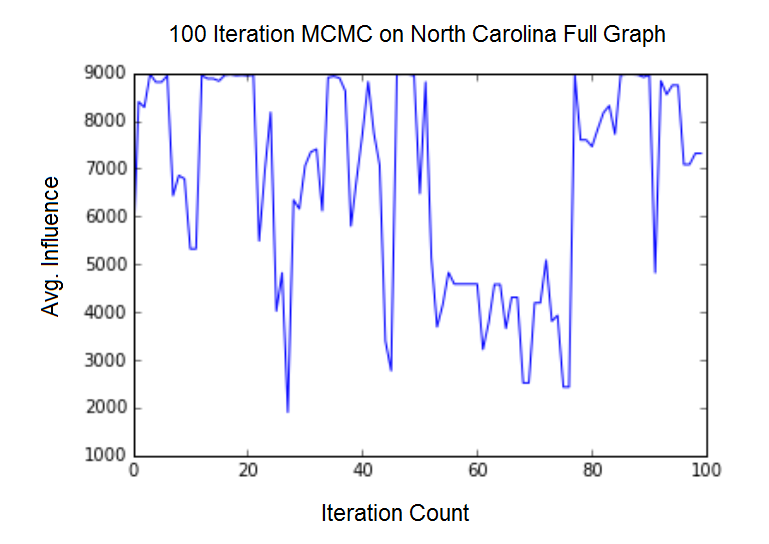
\includegraphics[scale=0.7]{nc_full_mcmc.png}
		
		Max influence = 8975.7
		
		Nodes (by hash): \texttt{u'9ki\_\-I7oW6YxnUZBCmxs5Q', u'GllP-lYGO1m61G4ly5fYTQ', u'iCePpGSAgAOSYZ9TkCQ09w'}
		
		All MCMC runs seem to max out around ~9000 influence...?
	
	
\end{document}